\section{Лекция 9 (13.04)}

\subsection{Учёт скошенности сетки в двумерной МКО-аппроксимации}
\subsubsection{Уточнённая аппроксимация нормальной производной}
Ключевым моментом для аппроксимации оператора Лапласа
методом конечных объёмов является выражение нормально производной
по грани конечного объёма.
До сих пор мы пользовались соотношением \cref{eq:fvm_dudn_dudc},
которая на скошенных сетках приводила к большим численным погрешностям
и не давала желаемый второй порядок аппроксимации (см. задачу из п.~\ref{sec:hw_fvm2d}).
Для устранения этого недостатка распишем нормальную производную по грани более точно.

Для двумерного случая распишем градиент $u$ в системе координат,
образованной еодиничными векторами нормали $\vec n$ и касательной $\vec s = (-n_y, n_x)$
к грани $\gamma_{ij}$ (см. рисунок \figref{fig:fvm_grid}):
$$
\nabla u = \dfr{u}{n}\vec n + \dfr{u}{s} \vec s.
$$
С помощью значений функции в точках коллокации $i$ и $j$
мы можем аппроксимировать производную
$$
\left.\dfr{u}{c}\right|_{\gamma_{ij}} = \frac{u_j - u_i}{h_{ij}} + O(h^2)
$$
в центре грани $\gamma_{ij}$ вторым порядком точности как симметричную разность.
Эта производная есть проекция градиента функции $u$ на
вектор $\vec c$. Тогда можно записать:
$$
\dfr{u}{c} = \nabla u \cdot \vec c = \dfr{u}{n} \vec n \cdot \vec c + \dfr{u}{s} \vec s \cdot \vec c
 = \dfr{u}{n} \cos(\vecangle{n}{c}) + \dfr{u}{s} \sin(\vecangle{n}{c}).
$$
Отсюда выразим искомую производную
\begin{equation}
\label{eq:fvm_dudn_div}
\dfr{u}{n} = \dfr{u}{c} \frac{1}{\cos(\vecangle{n}{c})} - \dfr{u}{s} \tan(\vecangle{n}{c}).
\end{equation}
Для записи аппроксимации второго порядка нормальной производной
необходимо с заданной точностью аппроксимировать производную по касательной к грани.
В двумерном случае введём вспомогательные точки $\vec c^{+}$  и $\vec c^{-}$ как
показано на рисунке (\ref{fig:fvm_skew_example}). Тогда в центре грани запишем искомую симметричную разность
$$
\dfr{u}{s} = \frac{u^{+} - u^{-}}{|\vec c^+ - \vec c^-|} + O(h^2).
$$
Тогда получим аппроксимацию второго порядка искомой производной:
\begin{equation}
\label{eq:fvm_dudn_upm}
\dfr{u}{n} \approx \frac{u_j - u_i}{|\vec c_j - \vec c_i|} \frac{1}{\cos(\vecangle{n}{c})} - \frac{u^{+} - u^{-}}{|\vec c^+ - \vec c^-|}  \tan(\vecangle{n}{c}).
\end{equation}
Точки $c^{\pm}$ не являются точками коллокации, поэтому значения $u^{\pm}$ явно
присутствовать в аппроксимационной схеме не могут. Однако, их можно проинтерполировать
через значения $u$ в точках коллокации.

\subsubsection{Интерполяция значения функции во вспомогательных точках}
Для простой линейной интерполяции функции, заданной на двумерной плоскости,
необходимо три узловые точки, не лежащие на одной прямой.
Пусть двумя из этих трёх точек будут уже обозначенные $\vec c_i$ и $\vec c_j$.
Третью точку $\vec c_k$ будем выбирать из коллокации, 
соседних с временной точкой:
центров ячеек и центров граничных граней, которые содержат точку $\vec c^-$.

\begin{figure}[h!]
\centering
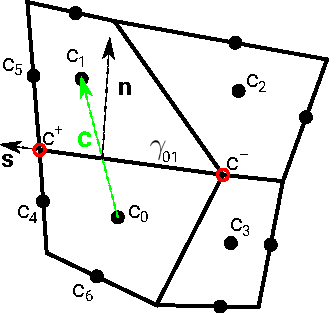
\includegraphics[width=0.25\linewidth]{fvm_skew_example.pdf}
\caption{Пример расположения вспомогательных точек (показаны красными кругами) для аппроксимации производной по грани}
\label{fig:fvm_skew_example}
\end{figure}

На примере с рис.~\ref{fig:fvm_skew_example} для точки $\vec c^-$ соседними будут точки $c_0, c_1, c_2, c_3$.
Точки $\vec c_0$ и $\vec c_1$ -- это первые две точки интерполяции (узлы $i$ и $j$ в предыдущих обозначениях).
Третью точку выберем как ближайшую к $\vec c^-$ из остальных, а именно $c_3$.
Для точки $\vec c^+$ третьей точкой будет $c_4$, выбранная аналогичным образом
из набора $c_0, c_1, c_4, c_5$.

Отметим, что для написания надёжного кода необходимо удостовериться,
что выбранная третья точка не лежит на одной прямой с двумя первыми.
И если лежит, то необходимо выбрать следующего кандидата.
А если кандидатов больше нет, то поиск необходимо продолжить
среди несоседних точек коллокации.

После того, как три узловые точки интерполяции
выбраны можно выразить вспомогательные значения
\begin{align*}
&u^- = C^-_i u_i + C^-_j u_j + C^-_k u_k,\\
&u^+ = C^+_i u_i + C^+_j u_j + C^+_s u_s,
\end{align*}
где коэффициенты интерполяции $C$ вычисляются следуя формуле
\cref{eq:simplex_interp_2d}. Например,
$$
C^-_i = \frac{|\triangle_{jk-}|}{\triangle_{ijk}|} =
\frac{
(\vec c_k - \vec c_j)\times(\vec c^- - \vec c_j)
}{
(\vec c_j - \vec c_i)\times(\vec c_k - \vec c_i)
}
$$
Подставив полученные интерполяционные соотношения в \cref{eq:fvm_dudn_upm},
получим аппроксимацию нормальной производной в виде линейную формы
\begin{equation}
\label{eq:fvm_dudn_linform}
\dfr{u}{n} \approx C_i u_i + C_j u_j + C_k u_k + C_s u_s.
\end{equation}
Коэффициенты которой равны
\begin{align*}
&C_i = -w_1 - (C_i^+ - C_i^-)w_2,
\\
&C_j = w_1 - (C_j^+ - C_j^-)w_2,
\\
&C_k = C_k^- w_2,
\\
&C_s = -C_s^+ w_2,
\\
&w_1 = \frac{1}{|\vec c_j - \vec c_i|\cos(\vecangle{n}{c})},
\\
&w_2 = \frac{\tan(\vecangle{n}{c})}{|\vec c^+ - \vec c^-|}
\end{align*}

\subsubsection{Производная по границе}
Из-за использования расширенного набора точек коллокации, 
процедура аппроксимации нормальной производной по граничной грани
ничем не отличается от аналогичной процедуры
для внутренней грани.
Так для точки коллокации $\vec c_4$
линейная форма, аппроксимирующая нормальную производную,
будет содержать значения $u_4, u_0, u_6, u_1$,
последние два из которых используются для интерполяции
вспомогательных точек.

Рассмотрим условие третьего рода \cref{eq:fvm_bc3} на стенке, соответсвующей
индексу коллокации $j$, соседней с ячейкой $i$.
C учётом \cref{eq:fvm_dudn_linform} получим:
\begin{equation*}
\dfr{u}{n} = C_i u_i + C_j u_j + C_k u_k + C_s u_s = \alpha u_j + \beta,
\end{equation*}
тогда $j$-ое уравнение СЛАУ будет иметь вид
\begin{equation}
\label{eq:fvm_bc3_skew_slae}
C_i u_i + (C_j - \alpha) u_j + C_k u_k + C_s u_s = \beta.
\end{equation}

\subsubsection{Сборка СЛАУ для уравнения Пуассона}
Рассмотрим процедуру сборки системы линейных уравнений для решения уравнения Пуассона.
Будем использовать цикл по граням по аналогии с \cref{eq:fvm_assem_internal}.
Ключевым моментом алгоритма будет являтся вычисление линейной формы
вида \cref{eq:fvm_dudn_linform}.
Отметим, что цикл по внутренним \cref{eq:fvm_assem_internal} и граничным \cref{eq:fvm_assem_bc_extended} граням
можно объединить в один цикл по всем граням. При этом следует
иметь ввиду, что этот цикл собирает уравнение внутри конечного объема
\cref{eq:fvm_pois_int}, и поэтому вносит изменения только
в строки, соответствующие центрам ячеек.
\begin{equation}
\label{eq:fvm_assem_internal_skew}
\begin{array}{ll}
\textbf{for } s \in\textrm{faces}                                & \textrm{-- цикл по всем граням}\\ 
\qquad i,j,k,s = \textrm{dn\_cells(s)}                           & \textrm{-- индексы точек коллокации для аппроксимации $\dsfr{u}{n}$}\\
\qquad v_i,v_j,v_k,v_s = \textrm{dn\_coefs(s)}                   & \textrm{-- коэф-ты линейной формы для аппроксимации $\dsfr{u}{n}$ }\\
\qquad a = \textrm{face\_area}(s)                                & \textrm{-- площадь грани}\\
\qquad \textbf{if } i \textrm{ is cell center }                  & \textrm{-- если $i$ -- коллокация для центра ячейки}\\
\qquad \qquad A_{ii} \minuseq  a\,v_i;                           & \textrm{-- $i$-ая строка матрицы (против нормали к грани)}\\ 
\qquad \qquad A_{ij} \minuseq  a\,v_j;                           & \\ 
\qquad \qquad A_{ik} \minuseq  a\,v_k;                           & \\
\qquad \qquad A_{is} \minuseq  a\,v_s;                           & \\
\qquad \textbf{endif}                                            & \\
\qquad \textbf{if } j \textrm{ is cell center }                  & \textrm{-- если $j$ -- коллокация для центра ячейки}\\
\qquad \qquad A_{ji} \pluseq a\,v_i;                             & \textrm{-- $j$-ая строка матрицы (по нормали к грани)}\\ 
\qquad \qquad A_{jj} \pluseq a\,v_j;                             & \\ 
\qquad \qquad A_{jk} \pluseq a\,v_k;                             & \\
\qquad \qquad A_{js} \pluseq a\,v_s;                             & \\
\qquad \textbf{endif}                                            & \\
\textbf{endfor}                                                  & \\
\end{array}
\end{equation}

В случае, если используются граничные условия второго или третьего рода,
та же процедура должна быть использована для выражения на границах \cref{eq:fvm_bc3_skew_slae} по аналогии с 
\cref{eq:fvm_assem_bc3_extended}.
\begin{equation*}
%\label{eq:fvm_assem_bc3_skew_extended}
\begin{array}{ll}
\textbf{for } s \in\textrm{bnd3}                         & \textrm{-- грани с условиями третьего рода}\\ 
\qquad i,j,k,s = \textrm{dn\_cells(s)}                   & \textrm{-- индексы точек коллокации для аппроксимации $\dsfr{u}{n}$}\\
\qquad v_i,v_j,v_k,v_s = \textrm{dn\_coefs(s)}           & \textrm{-- коэф-ты линейной формы для аппроксимации $\dsfr{u}{n}$ }\\
\qquad \textbf{if } j \textrm{ is cell center}           & \\
\qquad \qquad \textrm{swap}(i, j)                        & \textrm{-- переворачиваем нормаль. Теперь $j$ -- коллокация по грани} \\
\qquad \qquad v_i = -v_i, \quad v_j = -v_j               & \\
\qquad \qquad v_k = -v_k, \quad v_s = -v_s               & \\
\qquad \textbf{endif}                                    & \\
\qquad A_{ji} = C_i, \qquad A_{jj} = C_j-\alpha          & \\
\qquad A_{jk} = C_k, \qquad A_{js} = C_s                 & \\
\qquad b_{j} = \beta                                     & \\
\textbf{endfor}                                          & \\
\end{array}
\end{equation*}

\subsection{Задание для самостоятельной работы}
Решить двумерную задачу Пуассона с граничными условиями первого рода, аналогичную \ref{sec:hw_fvm2d},
но использовать поправку на скошенность.
Провести расчёт на сгущающихся сетках
и проиллюстрировать порядок аппроксимации
для структурированной, pebi и скошенной сетки.
Сравить графики сходимости с аналогичными, полученными в п.~\ref{sec:hw_fvm2d}.

\paragraph{Рекоммендации к программированию}
Для вычисления линейной формы \cref{eq:fvm_dudn_linform}
использовать класс \cvar{FvmLinformFacesDn}
из файла \ename{fvm/fvm_assembler.hpp}.

Объект этого класс необходимо собрать на этапе инициализации задачи.
Далее линейные формы для заданной грани вычисляются вызовом метода
\cvar{FvmLinformFacesDn::linear_combination(size_t iface)}.
Этот метод возвращает упорядоченную линейную комбинацию
из четырех (для двумерной задачи) слагаемых.
Получение индексов и коэффициентов линейной формы согласно алгоритму
\cref{eq:fvm_assem_internal_skew} осуществляется следующим образом
\begin{cppcode}
FvmLinformFacesDn faces_dn(grid);
for (size_t iface=0; iface < grid.n_faces(); ++iface){
	auto linform = faces_dn.linear_combination(iface);
	size_t i = linform[0].first;
	size_t j = linform[1].first;
	size_t k = linform[2].first;
	size_t s = linform[3].first;
	double vi = linform[0].second;
	double vj = linform[1].second;
	double vk = linform[2].second;
	double vs = linform[3].second;
}
\end{cppcode}


